% !TEX program = xelatex
% Build from this folder: xelatex -interaction=nonstopmode -halt-on-error squeezing_report_v7.tex
% Run twice. Figures: analyze_squeezing_v7.py, refine_squeezing_v7.py, distributed_squeezing_v7.py.
\documentclass[11pt,a4paper]{article}
\usepackage{kotex}
\setmainhangulfont[ItalicFont={Malgun Gothic}]{Malgun Gothic}
\setsanshangulfont[ItalicFont={Malgun Gothic}]{Malgun Gothic}
\usepackage{amsmath,amssymb,bm}
\usepackage{graphicx,booktabs,longtable,tabularx,array}
\usepackage[margin=2.15cm]{geometry}
\usepackage{caption,enumitem,xcolor,fancyhdr}
\PassOptionsToPackage{obeyspaces}{url}
\usepackage[hidelinks]{hyperref}
\renewcommand{\contentsname}{목차}
\renewcommand{\abstractname}{요약}
\renewcommand{\figurename}{그림}
\renewcommand{\tablename}{표}
\renewcommand{\refname}{참고문헌}
\hypersetup{pdftitle={85Rb FWM: squeezing optima and experimental comparison},pdfauthor={GABES}}
\definecolor{navy}{HTML}{183B56}
\definecolor{teal}{HTML}{176B87}
\definecolor{amber}{HTML}{8B5421}
\definecolor{pale}{HTML}{F0F5F7}
\pagestyle{fancy}
\fancyhf{}
\lhead{\small GABES / $^{85}$Rb FWM}
\rhead{\small 스퀴징 이론과 실험 비교 · v7}
\cfoot{\thepage}
\setlength{\headheight}{15pt}
\setlength{\emergencystretch}{3em}
\setlength{\parskip}{4pt}
\setlength{\parindent}{0pt}
\setlist[itemize]{leftmargin=1.5em,itemsep=2pt,topsep=3pt}
\setlist[enumerate]{leftmargin=1.8em,itemsep=3pt,topsep=3pt}
\captionsetup{font=small,labelfont=bf}
\renewcommand{\topfraction}{.92}
\renewcommand{\bottomfraction}{.85}
\renewcommand{\textfraction}{.07}
\renewcommand{\floatpagefraction}{.82}
\setcounter{topnumber}{4}
\setcounter{totalnumber}{5}
\raggedbottom
\newcolumntype{Y}{>{\raggedright\arraybackslash}X}
\newcolumntype{P}[1]{>{\raggedright\arraybackslash}p{#1}}
\newcommand{\dB}{\,\mathrm{dB}}
\newcommand{\MHz}{\,\mathrm{MHz}}
\newcommand{\GHz}{\,\mathrm{GHz}}
\newcommand{\kHz}{\,\mathrm{kHz}}
\newcommand{\degC}{\,^{\circ}\mathrm C}
\newcommand{\Tr}{\operatorname{Tr}}
\newcommand{\ii}{\mathrm i}
\newcommand{\commit}[1]{\href{https://github.com/Shake2313/fwm-squeezing-app/commit/#1}{\texttt{#1}}}
\newcommand{\code}[1]{\nolinkurl{#1}}
\makeatletter
\let\tableinput\@@input
\setlength{\@fptop}{0pt}
\setlength{\@fpsep}{18pt}
\setlength{\@fpbot}{0pt plus 1fil}
\makeatother
\newcommand{\note}[1]{\par\smallskip\noindent\colorbox{pale}{\begin{minipage}{0.955\linewidth}#1\end{minipage}}\par\smallskip}
\graphicspath{{v7_science/}{./}}
\title{\textbf{$^{85}$Rb 사광파 혼합의 세기차 스퀴징}\\[8pt]
\large 최적 조건, 다변수 민감도 및 실험과의 정량 비교}
\author{GABES (Generic Atomic Bloch Equation Solver)}
\date{2026년 9월 8일 · 보고서 v7}
\begin{document}
\maketitle
\begin{abstract}
열 원자 증기에서 발생하는 사광파 혼합(FWM)의 세기차 스퀴징을 이득, 셀 내부
흡수, 검출 손실 및 기술잡음의 함수로 분석한다. 이상적 증폭기에서는 이득을
높일수록 스퀴징이 개선되지만, 분포된 흡수와 이득이 함께 작용하면 유한한
최적점이 생긴다. 이 차이를 출발점으로 이론상의 최적 조건, GABES 평균장
계산의 변수 의존성, 실제 실험에서 확인된 허용범위를 연결한다.

Gold reference인 Sim 등\cite{sim}의 입력 seed $8\,\mu$W와 두 출력
$111/109\,\mu$W만으로 분포 이득·흡수 모형을 제약하면 모형 내 적합 이득은
$G=16.03$, 이득을 끈 probe 투과도는 $T_s=0.821$이다. 스퀴징을 적합에
사용하지 않고 계산한 검출 IDS는 총효율의 정의에 따라 $-7.71$ 또는
$-7.82\dB$이며, 실측 $-7.8\dB$와 약 $0.09\dB$ 이내에서 정합한다.
Gold와 두 McCormick 실험의 실측 이득·효율을 이상적 손실식에 넣은 결과도
직접 IDS와 약 $0.03$--$0.16\dB$ 차이를 보인다. 이는 평균 광학량에 조건을
둔 양자모형의 설명력이며, 원자 입력만으로 이득과 잡음을 모두 예측한
독립 검증과는 구분한다.

GABES에는 gold 이득 $15$ 하나로 결합계수를 보정한 조건부 분석을 적용했다.
OPD, TPD, 온도, pump, seed, 빔 반경, 셀 길이와 교차각을 스캔하여
$0.5\dB$ 악화 경계와 TPD 재조정 효과를 구했다. 이득만을 잡음으로 환산하는
근사는 높은 이득 영역을 과도하게 선호하고 seed의 실험적 상·하한을 설명하지
못한다. 반면 분포 잡음 모형은 이득과 흡수의 공통 스케일에 대해 유한한
최적점과 허용구간을 준다. 실측 seed plateau, 에탈론 온도 안정도,
공간모드 손실과 저주파 산란 한계를 함께 제시하여 계산을 실험 운전 조건으로
옮길 때 필요한 제약을 정리한다.
\end{abstract}
\clearpage
\begingroup\small\setlength{\parskip}{0pt}\tableofcontents\endgroup
\clearpage

\section{대상 계와 비교 기준}
\subsection{무엇을 최적화하는가}
대상은 $^{85}$Rb D1 이중-$\Lambda$ 계에 강한 pump와 약한 coherent probe를
입사시켜 생성하는 probe--conjugate twin beam이다. 두 pump 광자가 서로
상관된 광자쌍으로 전환되므로, 각 빔이 큰 강도 요동을 가져도 두 광전류의
차는 shot-noise limit(SNL)보다 작아질 수 있다. 이 보고서에서 좋은 스퀴징은
정해진 RF 분석 주파수에서, 같은 검출 파워와 같은 전자 가중치로 교정한
SNL에 대한 세기차 잡음의 감소를 뜻한다.
\begin{equation}
 R(\Omega)=\frac{S_{i_s-wi_c}(\Omega)}{S_{\rm SNL}(\Omega;w)},\qquad
 S_{\rm IDS}=10\log_{10}R,\qquad S_{\rm SNL}=2e(I_s+w^2I_c).
 \label{eq:snl}
\end{equation}
마지막 식은 동일한 광전류 단위에서의 단측 PSD 규약이다. $w$는 전자
가중치이며 기본 비교는 $w=1$이다. $S_{\rm IDS}<0$이면 sub-shot noise다.
전자 배경의 차감 여부, 검출 대역폭, 광학 손실의 기준면이 달라지면 같은
장치에서도 보고되는 dB가 달라진다. 회귀 기울기로 상수 전자 배경을 제거한
IDS와 외부 광학 손실까지 역보정한 내부 IDS도 서로 다른 양이다.

\subsection{Gold 운전점과 주파수 규약}
주요 기준은 EOM 기반 단일 레이저로 $^{85}$Rb twin beam을 생성한
Sim 등\cite{sim}이다. 빔 크기는 $1/e^2$ 강도 반경으로 사용한다.
표~\ref{tab:gold}의 값은 실험의 반올림된 대표값이며, 서로 다른 그림의
gain과 power를 불확도 없는 하나의 정밀 데이터로 간주하지 않는다.

\begin{table}[htbp]\centering
\caption{Gold 기준 조건. $\eta$는 셀 이후 두 검출 채널에 동일하게 적용하는 총효율이다.}
\label{tab:gold}
\begin{tabularx}{\linewidth}{P{4.1cm}P{3.4cm}Y}
\toprule 변수 & 기준값 & 의미\\\midrule
OPD $\Delta_\nu$ / TPD $\delta_\nu$ & $0.90\GHz$ / $-8\MHz$ & pump / Raman detuning\\
셀 온도 / 길이 & $121\degC$ / $12.5$ mm & 원자 밀도와 상호작용 길이\\
Pump / seed 입력 & $600$ mW / $8\,\mu$W & 셀 입력 파워\\
Pump / probe 반경 & $530/330\,\mu$m & 계산의 conjugate 반경도 $330\,\mu$m\\
교차각 $\theta$ & $0.32^\circ$ & pump--probe 사이 각도\\
출력 probe / conjugate & $111/109\,\mu$W & 입력 대비 파워비 $13.875/13.625$\\
보고 probe gain & 약 $15$--$16$ & IDS 운전 및 gain scan의 대표값\\
직접 IDS & $-7.8\dB$ & slope 분석은 약 $-8.7\dB$\\
총 검출효율 & $0.865$ 또는 $0.8694$ & 원문 총손실 $13.5\%$ / 코드의 $.945\times.92$\\
\bottomrule
\end{tabularx}
\end{table}

실험 입력은 ordinary frequency $\Delta_\nu,\delta_\nu$로 표시하고,
Bloch 방정식에서는 $\Delta=2\pi\Delta_\nu$, $\delta=2\pi\delta_\nu$를 쓴다.
$\Delta_\nu$의 기준은 $F=2\to F'=3$ 전이이다. 본문의 red-seeded
Raman branch에서
\begin{align}
 \omega_s&=\omega_p-2\pi\nu_{\rm HF}+2\pi\delta_\nu,\qquad
 \nu_{\rm HF}=3.0357\GHz,\\
 \omega_c&=2\omega_p-\omega_s.
\end{align}
Probe의 광학 scan 좌표는 $\Delta_\nu-\nu_{\rm HF}+\delta_\nu$이다.
RF 분석 주파수 $\Omega/2\pi$와 TPD는 독립 변수다. TPD scan에서 성능 임계값으로 정한 허용구간은
레이저 detuning에 대한 조건이며, squeezing의 RF 대역폭을 뜻하지 않는다.

\subsection{계산과 측정의 연결}
비교에는 세 수준을 사용한다. 실측 이득과 효율을 넣은 이상적 증폭기 식은
손실이 관측 IDS의 규모를 설명하는지 확인한다. 두 평균 출력을 넣은 분포
이득·흡수 모형은 내부 vacuum 유입까지 포함해 IDS를 계산한다.
GABES의 원자 평균장 계산은 실험 입력을 바꿀 때 이득이 어떻게 변하는지 제공한다.
마지막 수준에 완전한 원자 잡음 계산이 아직 없으므로, GABES 스캔에는
명시적인 이상적 잡음 환산식을 적용한다.

앞의 두 모형은 관측값과의 물리적 정합성을, GABES 스캔은 보정한 운전점
주변의 조건부 민감도를, 문헌의 실제 변수 스캔은 장치가 달성한 운전
허용범위를 알려준다.

\section{이득·흡수·잡음으로 정해지는 스퀴징 함수}
\subsection{이상적 두 모드 증폭기와 검출 손실}
Reservoir가 없는 위상정합 증폭기의 입력--출력 관계는 위상을 선택하면
\begin{equation}
 \hat a_s'=\sqrt G\hat a_s+\sqrt{G-1}\hat a_c^\dagger,\qquad
 \hat a_c'=\sqrt G\hat a_c+\sqrt{G-1}\hat a_s^\dagger,\quad G\geq1.
\end{equation}
입력 probe가 광자수 $n_0$가 큰 coherent seed이고 conjugate 입력이 진공일 때,
자발 항에 비해 큰 seed 항만 남기면 $\bar n_s=Gn_0$,
$\bar n_c=(G-1)n_0$이다. 광자수 차가 보존되는 반면 SNL은 총출력에
비례하므로, 두 팔의 효율이 $\eta$로 같을 때
\begin{equation}
 R_{\rm id}(G,\eta)=1-\eta+\frac{\eta}{2G-1},\qquad R_{\rm floor}=1-\eta.
 \label{eq:ideal}
\end{equation}
$G=15$, $\eta=0.8694$에서 $S_{\rm id}=-7.943\dB$이며 무한 이득의
한계는 $-8.841\dB$다. 따라서 이 조건에서 이득을 무한히 높여 얻을 수 있는
추가 개선은 약 $0.90\dB$뿐이다. 이미 큰 이득을 확보했다면 광학 효율과
잡음 억제가 중요한 이유가 여기에 있다.
\begin{equation}
 \frac{\partial R_{\rm id}}{\partial G}=-\frac{2\eta}{(2G-1)^2},\qquad
 \frac{\partial R_{\rm id}}{\partial\eta}=-1+\frac1{2G-1}.
\end{equation}
Gold 기준의 국소 기울기는 gain 1 증가당 약 $-0.0559\dB$,
효율 1 percentage point 증가당 약 $-0.261\dB$다. 이 식 자체에는
유한한 최적 gain이 없다. 실험의 유한 최적점은 이득 증가와 함께 변하는
흡수·공간모드·기술잡음을 포함해야 설명된다.

\subsection{불균형 검출과 공분산}
서로 다른 효율 $\eta_s,\eta_c$를 허용하고 $A=\eta_sG$,
$B=\eta_c(G-1)$라 두면, 입력 seed 광자수로 나눈 leading-order
분산과 공분산은
\begin{align}
 V_s&=A[1+2\eta_s(G-1)],&
 V_c&=B[1+2\eta_c(G-1)],\\
 C_{sc}&=2\eta_s\eta_cG(G-1),&
 R_w&=\frac{V_s+w^2V_c-2wC_{sc}}{A+w^2B}.
 \label{eq:weighted}
\end{align}
전자 가중치를 바꾸면 분자의 상관항과 분모의 SNL을 함께 바꿔야 한다.
평균 광전류를 같게 만드는 $w_{\rm DC}=G/(G-1)$와 이상적 잡음을
최소화하는 $w_{\rm opt}=\sqrt{G/(G-1)}$는 같지 않다. 두 식은 동일한
검출효율을 가정한다. $G=15$에서는 각각 $1.0714$, $1.0351$이다.
후자는 이상적 모형에서 $-8.369\dB$를 주지만, 이를 $w=1$의 IDS와 같은
관측량으로 비교해서는 안 된다. 실제 입력의 공통 기술잡음이 크면 DC
cancellation 쪽으로 최적 가중치가 이동할 수 있다.

\subsection{분포 이득·흡수와 vacuum 유입}
셀 안에서 증폭과 흡수가 교대로 일어나는 계는 출구에서 한 번 손실을
적용하는 모형과 다르다\cite{mc08}. 앞부분의 흡수로 유입된 vacuum이
뒷부분에서 다시 증폭되기 때문이다. 차원 없는 좌표 $u=z/L$에서 두
amplitude quadrature의 drift를
\begin{equation}
 M_x=\begin{pmatrix}-a/2&r\\r&0\end{pmatrix},\qquad
 r=\operatorname{arcosh}\sqrt G,\qquad a=-\ln T_s
 \label{eq:mx}
\end{equation}
로 둔다. $G$는 흡수를 끈 내부 이득, $T_s$는 이득을 끈 probe의 셀
투과도다. 관측된 출력 이득 $G_s,G_c$와 구별된다.
Probe만의 vacuum absorption, 일정한 계수, pump 비고갈, 완전한 위상정합,
한 공간모드와 분석 대역 내 평탄한 응답을 가정한다.

위상 quadrature의 행렬 $M_p$는 $M_x$의 비대각 원소 부호를 바꾼다.
$\bm X=(x_s,x_c,p_s,p_c)^T$, vacuum covariance $V_0=I/2$에 대해
\begin{align}
 K&=\operatorname{diag}(M_x,M_p),\qquad D=\operatorname{diag}(a/2,0,a/2,0),\\
 \frac{dV}{du}&=KV+VK^T+D,\\
 V_{\rm out}&=EV_0E^T+\int_0^1e^{Ks}D e^{K^Ts}\,ds,\qquad E=e^K.
 \label{eq:cov}
\end{align}
외부 검출손실은 $L_\eta=\operatorname{diag}
(\sqrt{\eta_s},\sqrt{\eta_c},\sqrt{\eta_s},\sqrt{\eta_c})$를 이용해
$V_{\rm det}=L_\eta V_{\rm out}L_\eta^T+(I-L_\eta L_\eta^T)/2$로 도입한다.
단위 seed 진폭에 대한 출력을 $(A_s,A_c)^T=e^{M_x}(1,0)^T$라 두면
\begin{equation}
 R=\frac{2\bm q^TV_{\rm det}\bm q}{\eta_sA_s^2+w^2\eta_cA_c^2},\qquad
 \bm q=(\sqrt{\eta_s}A_s,-w\sqrt{\eta_c}A_c,0,0)^T.
 \label{eq:covids}
\end{equation}
이 식은 drift와 diffusion에서 분산·공분산을 계산한 뒤 평균 출력과 결합한다.
무흡수에서는 식~\eqref{eq:ideal}을 회복하며, 순수한 수동손실을 받은
coherent seed는 $R=1$을 유지한다.

\subsection{다변수·다중모드 함수}
실험 입력을
\begin{equation}
 \bm x=(\Delta_\nu,\delta_\nu,T,P_p,P_s,w_p,w_s,L,\theta,
 \eta_s,\eta_c,\Omega,w,\ldots)
\end{equation}
로 모은다. 일반적인 선형화 양자모형에서 $K(z,\Omega;\bm x)$는 응답을,
$D(z,\Omega;\bm x)$는 원자·손실 reservoir 잡음을, 검출벡터는 수집
공간모드와 전자계를 정한다. 따라서 구하는 함수는
\begin{equation}
 S_{\rm IDS}(\bm x)=10\log_{10}
 \left[\frac{\bm c^\dagger V_{\rm det}(\Omega;\bm x)\bm c}
 {S_{\rm SNL}(\bm x)}\right].
 \label{eq:multivar}
\end{equation}
같은 평균 출력이라도 $D$와 수집모드가 다르면 잡음은 달라진다.
한 실험에 대한 작은 잔차만으로 이들 미지량이 유일하게 결정되지는 않는다.

\section{이론상 최적점과 허용범위}
\subsection{Gold 출력으로 제약한 분포모형}
보고된 $111/109\,\mu$W를 셀 출력으로 간주하고 후단손실은 $\eta$로
별도 적용하였다. 이 평균 출력과 seed $8\,\mu$W로 정한
$(G_s,G_c)=(13.875,13.625)$에 두 계수를 적합하면
\begin{equation}
 G=16.0259,\qquad T_s=0.82116
\end{equation}
이다. 스퀴징을 적합에 넣지 않은 예측은 $\eta=.8694$에서
$-7.819\dB$, 원문의 총손실을 직접 쓴 $\eta=.865$에서
$-7.709\dB$다. 둘 다 실측 $-7.8\dB$와 가깝다.
다만 효율 규약만으로 약 $0.11\dB$가 바뀌므로, $0.02\dB$ 일치를
정밀한 예측 정확도로 해석하지 않는다. Gaussian 환산에서는 두 출력의 상대 광주파수 차($2\times10^{-5}$ 미만)를
무시했다. 반올림 전 파워, 동일 운전점
측정, 손실 기준면을 맞춘 데이터가 정밀도 평가에 필요하다.

\begin{figure}[htbp]\centering
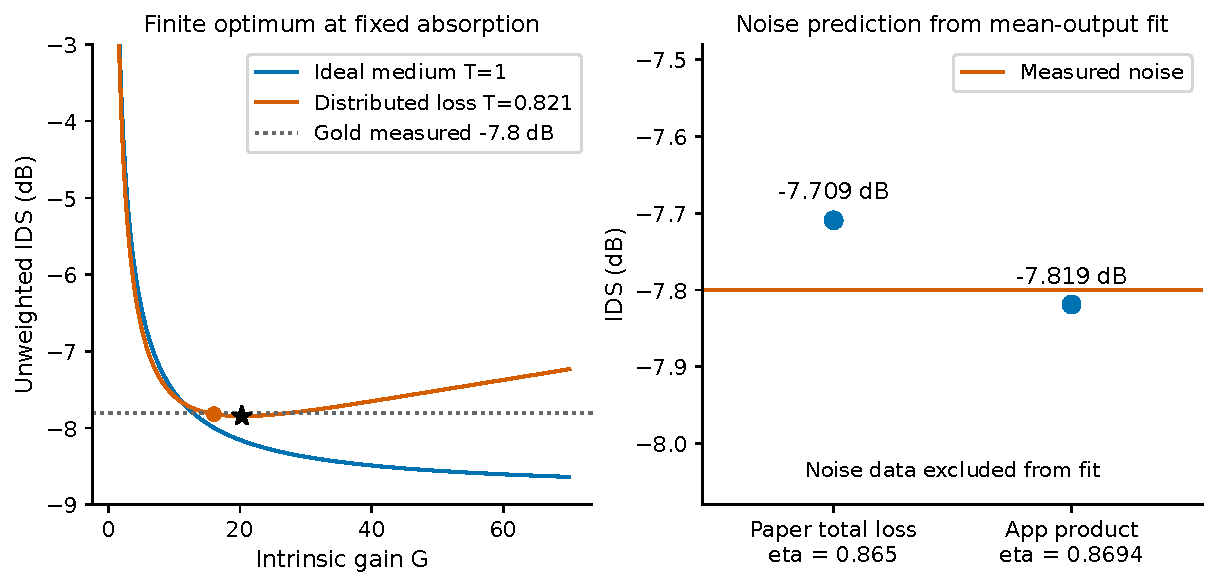
\includegraphics[width=.96\linewidth]{theory_gold_comparison.pdf}
\caption{Gold 평균 출력으로 제약한 분포모형, 이상적 손실모형과 실측 IDS.
분포모형은 스퀴징 값을 적합하지 않았다. 효율 정의와 반올림된 입력의
영향이 작은 잔차보다 클 수 있다.}
\label{fig:goldtheory}
\end{figure}

\subsection{고정하는 변수에 따른 최적점}
$\eta=.8694$, $w=1$에서 같은 분포모형에 세 가지 변화 방향을 적용했다.
표~\ref{tab:theoryopt}는 동일 함수의 서로 다른 단면이다.
실험의 온도 변화는 보통 이득과 흡수를 함께 바꾸므로, 고정 흡수의 최적
이득만으로 온도 최적점을 정할 수는 없다.

\begin{table}[htbp]\centering
\caption{분포모형의 조건부 최적점과 기준 $-7.819\dB$에서 $0.5\dB$ 이내인
연결구간. 모두 비가중 차분 $w=1$이다.}
\label{tab:theoryopt}
\begin{tabularx}{\linewidth}{P{4.4cm}P{3.1cm}Y}
\toprule 변화 방향 & 최적점 / IDS & $S\leq-7.319\dB$의 범위\\\midrule
내부 $G$; $T_s=.82116$ 고정 & $20.25$ / $-7.845$ dB & $7.58\leq G\leq63.68$\\
투과도 $T_s$; $G=16.026$ 고정 & $.93092$ / $-8.097$ dB & $.74697\leq T_s\leq1$\\
공통계수 $r\to xr,\ a\to xa$ & $x=1.0034$ / $-7.819$ dB & $.8037\leq x\leq1.2042$\\
\bottomrule
\end{tabularx}
\end{table}

고정 $T_s$에서 이득을 올리면 처음에는 쌍 상관이 커지지만, 이후에는
분포 흡수로 유입된 잡음의 재증폭이 불리하게 작용한다. 이 경쟁이 유한한
최적 $G$를 만든다. 고정 $G$에서 약간의 probe 흡수가 최적인 것은
비가중 차분에서 두 출력의 불균형과 분포 잡음이 함께 작용한 결과다.
이는 검출 전에 손실을 추가하라는 일반적 처방이 아니다.
외부 대칭손실은 식~\eqref{eq:ideal}에서 일관되게 IDS를 악화시킨다.

공통계수 $x$는 국소계수를 고정하고 셀 길이나 광학 깊이를 바꾸는 근사다.
기준 $x=1$이 최적점에 가까워, 단순한 이득 증가보다 이득과 흡수의 비를
개선하는 편이 유리하다. 온도는 Doppler 폭·충돌·population도 바꾸므로,
$x$의 약 $\pm20\%$ 범위를 그대로 온도 허용범위로 해석하지 않는다.

\begin{figure}[htbp]\centering
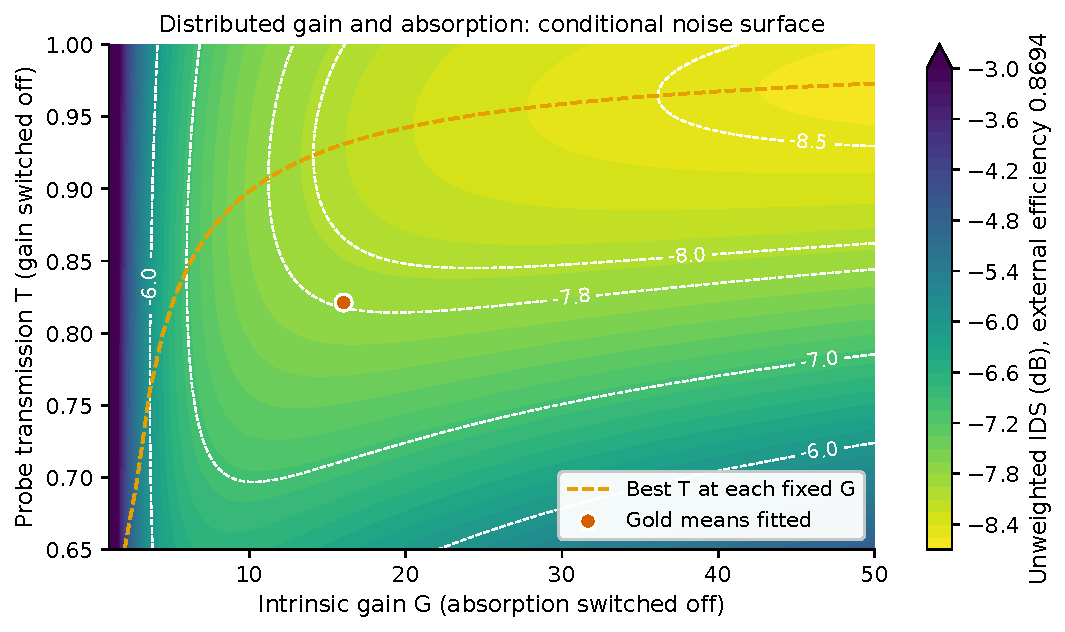
\includegraphics[width=\linewidth]{theory_gain_absorption.pdf}
\caption{내부 이득과 probe 흡수가 만드는 스퀴징 함수 및 단면.
표시된 이변수 영역의 최소는 이득 상한 경계에 있다. 표~\ref{tab:theoryopt}의
유한 최적점은 고정 흡수 또는 공통계수 변화라는 조건에 의존한다.}
\label{fig:ga}
\end{figure}

\subsection{손실·배경·seed 잡음의 공통 예산}
이상적인 동효율·비가중 검출에서 입력 seed의 초과 잡음을 $\xi$로 둔다.
이는 선택한 분석 주파수에서 입력 seed의 잡음 PSD/SNL$-1$이며,
해당 검출 대역의 초과 Fano factor에 대응한다. 독립 배경광을 제외한
twin-beam SNL로 정규화한 가산 잡음을 $\epsilon$이라 하면
\begin{equation}
 R=1-\eta+\eta\frac{1+\xi}{2G-1}+\epsilon.
 \label{eq:budget}
\end{equation}
쌍과 독립적인 coherent 광이 검출 총 SNL의 비율 $f$를 차지하면
$R_{\rm mix}=(1-f)R+f$다. $\epsilon$은 잡음 PSD의 비이고,
$f$는 총 SNL에 대한 기여비로 서로 다른 양이다.

\begin{table}[htbp]\centering
\caption{이상적 기준 $G=15,\eta=.8694,S_0=-7.943\dB$에서의 단일변수 예산.
다른 변수는 기준값으로 고정한다. 각 열의 상한을 동시에 사용할 수 없다.}
\label{tab:budget}
\begin{tabularx}{\linewidth}{P{5.2cm}YY}
\toprule 조건 & $+0.5\dB$ 이내 & $-7.8\dB$ 이하 유지\\\midrule
검출효율 $\eta$ 하한 & $0.84911$ & $0.86383$\\
이득 $G$ 하한 & $9.269$ & $12.794$\\
가산 잡음 $\epsilon$ 상한 & $0.019594$ SNL & $0.005379$ SNL\\
위 가산 잡음의 dB 값 & $-17.08\dB$ SNL & $-22.69\dB$ SNL\\
독립 coherent 광의 총 SNL 비율 $f$ & $2.334\%$ 이하 & $0.641\%$ 이하\\
입력 seed 초과 Fano factor $\xi$ & $0.654$ 이하 & $0.179$ 이하\\
전자차분 가중치 $w$ & $0.9822$--$1.0908$ & $0.9943$--$1.0776$\\
\bottomrule
\end{tabularx}
\end{table}

$-7.8\dB$ 유지에 쓸 수 있는 손실 여유는 총효율로 약 $0.557$
percentage point뿐이다. 배경광·전자 잡음·seed RIN이 공존하면 같은
여유를 나눠 쓴다. 국소적으로
\begin{equation}
 \delta R\simeq-\frac{2\eta}{(2G-1)^2}\delta G
 -\left(1-\frac1{2G-1}\right)\delta\eta
 +\frac{\eta}{2G-1}\xi+\epsilon+(1-R_0)f
\end{equation}
를 공통 상한과 비교한다. 변수마다 최대 공차를 배정한 직육면체는 일반적으로
전체 허용영역에 포함되지 않는다.

두 신호의 지연차도 상관을 낮춘다. 평탄한 실수 공분산을 가정하면
식~\eqref{eq:weighted}의 $C_{sc}$를 $C_{sc}\cos(\Omega\tau)$로
치환할 수 있다. Gold 이상기준에서 $500\kHz$를 평가하는 예로,
$0.5\dB$ 예산은 약 $12.6$ ns, $-7.8\dB$ 유지는 약 $6.6$ ns 이하의
잔여 지연차에 해당한다. 실제 공분산과 군지연 분산은 주파수별로 평가해야 한다.

\begin{figure}[htbp]\centering
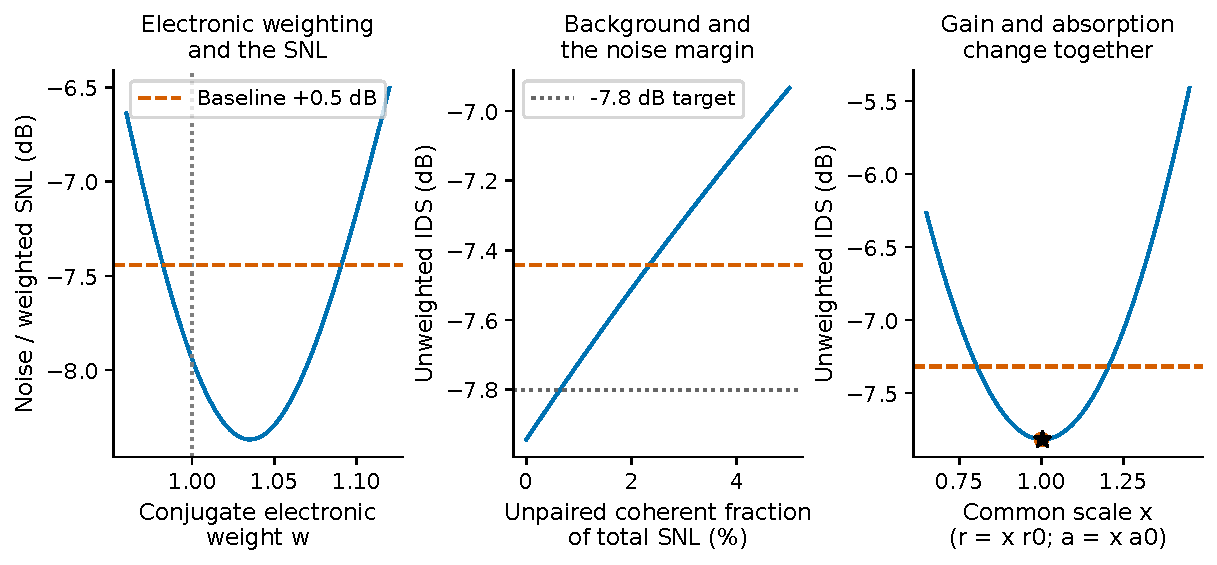
\includegraphics[width=\linewidth]{theory_tolerance.pdf}
\caption{이상적 검출모형의 잡음 예산과 분포모형의 민감도.
단일변수 상한은 공유 예산이다. 두 모형의 $0.5\dB$ 조건은 각각의 기준 IDS에
대한 것으로, 동일한 절대 임계값은 아니다.}
\end{figure}

\section{실험변수의 물리적 결합}
\subsection{OPD--TPD: 공명 위치와 세기}
원거리 detuning·약한 포화 근사에서는 Raman 결합이
$\Omega_{\rm eff}\propto\Omega_p\Omega_s/\Delta$,
광시프트가 $\delta_{\rm AC}\propto|\Omega_p|^2/\Delta$로 변한다.
OPD를 바꾸면 결합 세기와 최적 TPD가 함께 움직인다. 광시프트를
국소적으로 유지하는 조건은
\begin{equation}
 \delta\ln P_p-2\delta\ln w_p-\delta\ln|\Delta|\simeq0
\end{equation}
이다. 다준위·Doppler 평균·강한 pump에서는 정량식은 아니지만,
TPD 고정과 재조정에서 허용범위가 달라지는 원인을 설명한다.

\subsection{Pump 파워--빔 반경}
Gaussian beam의 중심 강도와 Rabi 주파수는
\begin{equation}
 I_{p,0}=\frac{2P_p}{\pi w_p^2},\qquad
 |\Omega_p|\propto\frac{\sqrt{P_p}}{w_p}.
\end{equation}
Gold 중심 강도는 약 $136\,\mathrm{W/cm^2}$이다. 국소 drive를
보존하는 일차 보상은 $\delta P_p/P_p\simeq2\delta w_p/w_p$다.
그러나 반경은 교차영역, 수집률, 원자 통과시간, Rayleigh 길이
$z_R=\pi w_p^2/\lambda$도 바꾼다. 같은 강도가 같은 IDS를 보장하지 않는다.

\subsection{온도--셀 길이}
광학 깊이의 주요 인자는 $\mathrm{OD}\propto N(T)L$이다.
밀도 증가는 이득을 높이지만 흡수·충돌·형광도 늘린다.
일정한 광학 깊이의 국소 조건은
\begin{equation}
 \delta\ln L\simeq-\frac{d\ln N}{dT}\delta T.
\end{equation}
코드의 증기밀도식은 $121\degC$에서 $d\ln N/dT\simeq0.05836$
K$^{-1}$, 온도 1°C 상승에 약 $5.99\%$ 밀도 증가를 준다.
같은 $NL$이어도 Doppler 폭·충돌률은 다르고, 셀 길이는
$\Delta k_zL$과 beam walk-off를 바꾼다. 온도와 길이는 주요 보상변수지만
완전히 하나의 곱으로 환원되지는 않는다.

\subsection{교차각--RF 평가 주파수}
등방 원자속도의 성분 표준편차 $\sigma_v=\sqrt{k_BT/m}$에 대해,
두 광장의 Raman Doppler 폭은
\begin{equation}
 \sigma_{\delta_\nu}=\frac{\sigma_v}{2\pi}
 \sqrt{(k_p-k_s\cos\theta)^2+(k_s\sin\theta)^2}.
 \label{eq:angle}
\end{equation}
Gold에서는 약 $1.380\MHz$로, 횡방향 성분이 약 $1.380\MHz$,
축방향이 약 $5.85\kHz$이다. 공선에서도 광주파수 차로 약 $1.99\kHz$가
남는다. 이는 RMS 폭이며 스퀴징 FWHM이나 허용 TPD 폭은 아니다.
작은 각도는 운동 dephasing과 위상 불일치를 줄이지만 pump 산란의
공간분리를 어렵게 한다. Wu 등은 약 $0.3^\circ$에서 $0.5^\circ$로
넓혀 이득·대역 일부를 희생하고 저주파 pump 산란을 줄였다\cite{wu}.
최적 각도는 평가 RF와 pump 제거계에 결합된다.

\subsection{Seed--검출 배경--spectral purity}
이상적인 bright-seed 식의 정규화 IDS는 seed 파워와 무관하다.
실제로 약한 seed에서는 고정 전자 잡음의 상대 기여가 커지고, 강한 seed에서는
원자 포화·pump 고갈·기술잡음이 증가한다. 국소 근사
\begin{equation}
 R(P_s)\simeq R_q+\frac{A_{\rm el}}{P_s}+B_{\rm tech}P_s,\qquad
 P_{s,*}=\sqrt{A_{\rm el}/B_{\rm tech}}
\end{equation}
는 양쪽 한계가 생기는 이유를 보여준다. 계수는 장치와 RIN에 의존하므로
미측정 계수를 넣어 gold의 최적 seed를 수치화하지 않는다.
EOM carrier와 불필요 sideband는 셀에서 각기 다른 증폭·흡수를 겪는다.
셀 입력의 불필요 광 비율을 표~\ref{tab:budget}의 검출면 비율 $f$로
직접 대체해서는 안 된다.

\section{GABES의 다변수 조건부 예측}
\subsection{평균장과 계산 조건}
GABES는 4준위 Bloch 계의 finite-seed Floquet 응답을 속도 평균하고,
probe--conjugate Maxwell 전파를 구한다. 원자상태는 $\Tr\rho=1$이며
열평형 population을 외부에서 중복 적용하지 않는다. Transit reset은
\begin{equation}
 \mathcal L_t\rho=\gamma_t(\rho_{\rm th}\Tr\rho-\rho),\quad
 \rho_{\rm th}=\operatorname{diag}(5/12,7/12,0,0),\quad
 \gamma_t=2\pi\times100\kHz
\end{equation}
로 두었다. 외부 결합에는 구조계수 $1/12$와 residual $\ell$이 들어간다.
$\ell$은 독립 측정된 원자상수가 아닌 유효계수다.

전파에는 주파수별 vacuum 파수와 기하학적 위상 불일치를 쓴다.
대칭 mismatch gauge의 장
$(E_se^{-\ii\Delta k_zz/2},E_c^*e^{+\ii\Delta k_zz/2})^T$에 대해
\begin{equation}
 M_E=\begin{pmatrix}
 \ii k_s\chi_{ss}/2-\ii\Delta k_z/2&\ii k_s\chi_{sc}/2\\
 -\ii k_c\chi_{cs}^*/2&-\ii k_c\chi_{cc}^*/2+\ii\Delta k_z/2
 \end{pmatrix},\quad \Delta k_z=2k_p-(k_s+k_c)\cos\theta .
\end{equation}
$k_j=\omega_j/c$이고 $\chi$는 무차원 물리적 감수율이다. 감수율의
분산은 위상 불일치에 다시 넣지 않는다. Ultra는 64구간의 교차 profile과
근사적인 pump-budget 감소를 포함한다.

주 계산은 gold 조건, 표준 red-seeded branch, Ultra, $N_F=3$을 썼다.
속도 간격은 5 m/s, cutoff는 $4\sigma_v$이며, TPD
$-80$--$120\MHz$를 $2\MHz$ 간격으로 스캔했다. 각 scan의 전체 구간에서
$N_F=2$와 비교하여 주 분석의 206개 scan 모두 Floquet 수렴 판정을 통과했다.
기준과 허용경계의 추가 정밀화는 2.5 m/s, $5\sigma_v$를 사용했고, 145회
평가 모두 판정을 통과했다. Gold gain은 정밀화로 약 $0.0087\%$,
조건부 IDS는 약 $0.000073\dB$ 변했다. 이는 선택한 일차원 모델 내부의
수치 검사다.

\subsection{Gold 이득의 일점 보정}
기본 $\ell=.74$는 gold에서 $G_s\simeq394.3$, $G_c\simeq396.5$를
주어 실측 $G_s\simeq15$보다 약 26배 크다. 이에 \textbf{probe 이득 15
한 개만} 이용하여 $\ell=0.42505$로 보정했다. 그러면
$G_s=15.000$, $G_c=14.157$이다. 스퀴징과 다른 운전점의 값·기울기는
보정에 사용하지 않았다. 다음 식을 GABES 그림의 목적함수로 삼았다.
\begin{equation}
 S_{\rm cond}(\bm x)=10\log_{10}
 \left[1-\eta+\frac{\eta}{2G_s^{\rm GABES}(\bm x;\ell_*)-1}\right],
 \qquad G_s^{\rm GABES}\geq1.
 \label{eq:conditional}
\end{equation}
이 환산은 $G_c=G_s-1$인 이상적 상관을 가정한다. GABES의 실제 $G_c$에서
원자 공분산을 계산한 값은 아니다. $G_s<1$인 수동영역에는 적용하지 않는다.
기준은 $S_0=-7.943\dB$, 허용 임계값은 $S_0+0.5=-7.443\dB$다.

\subsection{OPD--TPD와 온도의 결합}
그림~\ref{fig:maps} 왼쪽은 OPD--TPD 면, 오른쪽은 각 OPD·온도에서 TPD를
다시 맞춘 최소값이다. TPD 고정 단면에서 민감한 변수도 TPD를 바꾸면
이득이 큰 다른 지점으로 보상할 수 있다. 각 변수를 독립 공차로 취급하기
어려운 이유를 이 지도에서 확인할 수 있다.
\begin{figure}[htbp]\centering
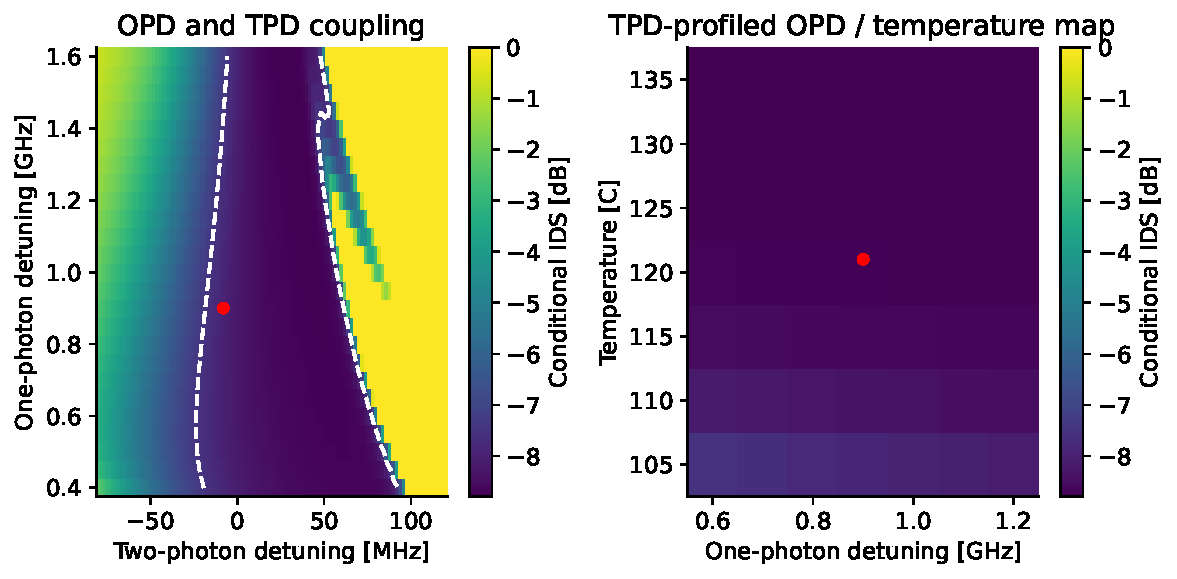
\includegraphics[width=\linewidth]{coupled_maps.pdf}
\caption{Gold 이득을 일계수로 보정한 GABES의 조건부 IDS.
왼쪽 흰 선은 $-7.443\dB$이고, 오른쪽은 TPD를 탐색 구간 안에서 재조정한다.
붉은 점은 gold 기준이다. 잡음은 식~\eqref{eq:conditional}로 환산한다.}
\label{fig:maps}
\end{figure}

다른 gold 변수를 고정하고 TPD를 정밀 탐색한 최소는
$\delta_\nu=46.25\MHz$, $G_s=222.10$, $S_{\rm cond}=-8.77582\dB$였다.
OPD $0.6$--$1.2\GHz$, 온도 $105$--$135\degC$의 이변수 주 격자에서는
$(1.2\GHz,135\degC,26\MHz)$가 $-8.83940\dB$로 최선이었다.
OPD·온도 모두 탐색 경계이므로 유한한 내부 최적점이 아니다.

이 고밀도 점은 small-signal gain 약 28,907에서 구간 pump 처리 후
약 18,457, 최종 cap 후 약 12,370으로 변한다. 마지막 cap만으로 약
33\% 감소한다. 반면 gold 기준의 최종 cap 영향은 약 0.035\%이다.
높은 이득의 지도 최소는 이상적 손실 floor $-8.84057\dB$에 접근한 결과로,
실험 운전점을 지시하지 않는다. 분포 잡음을 넣은 표~\ref{tab:theoryopt}의
유한 최적점과는 최적화하는 함수가 다르다.

\subsection{단일변수 허용폭과 TPD 재조정}
각 허용구간은 gold 기준점을 포함하고
$S_{\rm cond}\leq S_0+0.5\dB$인 \textbf{연결구간}이다.
재조정 TPD에도 같은 gold 임계값을 적용했다. 각 재조정점의 최소값에
별도로 $0.5\dB$를 더하지 않았다.
\begin{figure}[htbp]\centering
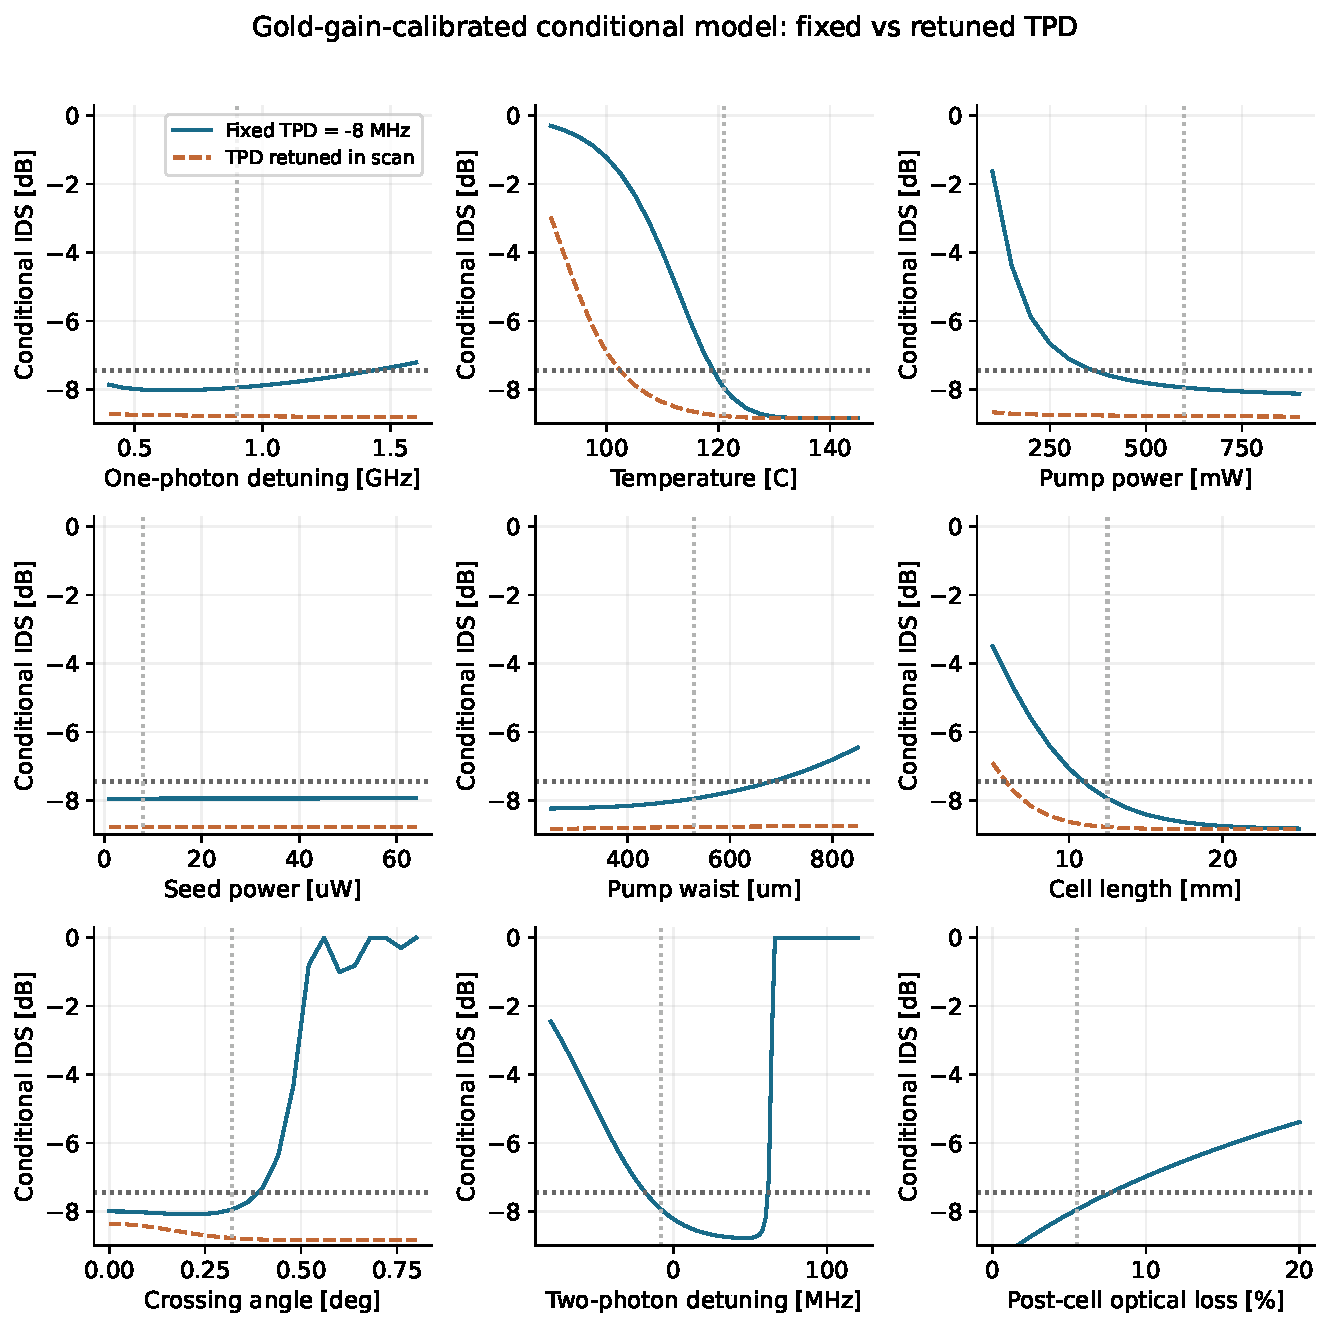
\includegraphics[width=.99\linewidth]{tolerance.pdf}
\caption{TPD $-8\MHz$ 고정(청색)과 탐색 구간 내 재조정(주황)의 단일변수
조건부 IDS. 수평 점선은 공통 임계값, 수직 점선은 gold 기준이다.
Seed의 평탄성과 높은 이득 쪽의 포화는 이상적 잡음 환산의 성질을 반영한다.}
\label{fig:tol}
\end{figure}

\begin{table}[htbp]\centering\small
\caption{조건부 $0.5\dB$ 허용구간. ``끝''은 탐색 끝에 걸렸다는 뜻이며
물리적 한계를 찾은 값이 아니다. 고정 TPD 교차경계는 세분화했고,
재조정 구간은 주 격자의 보간 근사다.}
\label{tab:codetol}
\begin{tabularx}{\linewidth}{P{3.1cm}P{2.8cm}P{4.2cm}Y}
\toprule 변수(기준) & 탐색범위 & TPD 고정 허용구간 & TPD 재조정\\\midrule
OPD ($.90\GHz$) & $.40$--$1.60$ & $.40$ (끝)--$1.4327$ & 전체 탐색범위\\
온도 ($121\degC$) & $90$--$145$ & $119.037$--$145$ (끝) & 약$102.4$--$145$ (끝)\\
Pump ($600$ mW) & $100$--$900$ & $361.84$--$900$ (끝) & 전체 탐색범위\\
Seed ($8\,\mu$W) & $1$--$64$ & 전체 탐색범위 & 전체 탐색범위\\
Pump 반경 ($530\,\mu$m) & $250$--$850$ & $250$ (끝)--$682.88$ & 전체 탐색범위\\
셀 길이 ($12.5$ mm) & $5$--$25$ & $10.898$--$25$ (끝) & 약$5.88$--$25$ (끝)\\
교차각 ($.32^\circ$) & $0$--$.8$ & $0$ (끝)--$.39053$ & 전체 탐색범위\\
외부 광학손실 ($5.5\%$) & $0$--$20\%$ & $0$--$7.71\%$ & QE $=.92$ 고정\\
\bottomrule
\end{tabularx}
\end{table}

TPD 자체는 다른 변수를 모두 고정한 상태에서
\begin{equation}
 -18.409\MHz\leq\delta_\nu\leq61.545\MHz
\end{equation}
가 허용 연결구간이다. 기준 $-8\MHz$ 대비 허용 drift는
$-10.409/+69.545\MHz$로 비대칭이다. 기준이 이 목적함수의 최적점이
아니기 때문에 대칭 공차로 바꾸면 정보를 잃는다.

이 모델에서는 온도를 낮추는 여유가 약 1.96°C로 작고, TPD를 함께 맞추면
허용영역이 크게 달라진다. Pump와 빔 반경은 강도 방향으로 결합하고,
각도도 TPD 보상을 받는다. 반면 seed $1$--$64\,\mu$W를 모두 허용하는
결과는 검출 배경과 포화의 실제 한계를 충분히 포함하지 못한다.
또한 출력 gain의 하한 처리가 수동영역을 $G_s=1$로 올리는 구간이 있어,
그림의 0 dB 평탄부를 실제 원자 잡음 예측으로 읽지 않는다.

\subsection{동시 drift와 제어 가능한 방향}
근방의 함수는
\begin{equation}
 S(\bm x_0+\bm u)\simeq S_0+\bm g^T\bm u+\tfrac12\bm u^TH\bm u
\end{equation}
로 전개된다. 기준이 최적점이 아니면 일차항 때문에 상·하한이 비대칭이다.
외란 $\bm u$와 조절변수 $\bm v$를 구분하고, 조절 방향이 국소 최적이며
$H_{vv}$가 양정치라면 재조정 후 곡률은
\begin{equation}
 H_{\rm prof}=H_{uu}-H_{uv}H_{vv}^{-1}H_{vu}
\end{equation}
이다. TPD 추종으로 허용영역이 넓어지는 효과가 교차항에 대응한다.
이번 다봉형 scan은 직접 최소화를 사용했으며, 하나의 Hessian으로
넓은 범위를 외삽하지 않았다. 먼 TPD 가지로의 이동에는 실제 lock이
연속적으로 따라갈 수 있는지도 추가 검증해야 한다.

\section{문헌과 이론의 정량 비교}
\subsection{동일 관측량으로 비교할 수 있는 실험}
\code{references/fwm_squeezing_paper_parameters.csv}의 10개 논문을
출발점으로 측정방식·손실정의·운전점을 일차자료에서 확인했다.
표~\ref{tab:direct}는 실측 이득과 총효율이 비교적 명확한 직접 IDS 세 사례다.
각 실험의 값을 식~\eqref{eq:ideal}에 대입한 결과다.
\begin{table}[htbp]\centering
\caption{실측 이득을 입력한 이상적 손실식의 IDS 비교.
잔차는 실측 minus 계산이다. 원자 이득의 독립 예측을 평가하는 표는 아니다.}
\label{tab:direct}
\begin{tabularx}{\linewidth}{P{3.6cm}P{2.4cm}P{2cm}P{2.8cm}Y}
\toprule 문헌 & $G$, $\eta$ & 실측 dB & 계산 dB & 잔차 dB\\\midrule
Sim 2025\cite{sim} & $15$--$16$, $.865$ & $-7.8$ & $-7.830$--$-7.881$ & $+.030$--$+.081$\\
McCormick 2007\cite{mc07} & $4$, $.656$ & $-3.5$ & $-3.588$ & $+.088$\\
McCormick 2008\cite{mc08} & $9$, $.90$ & $-8.0$ & $-8.155$ & $+.155$\\
\bottomrule
\end{tabularx}
\end{table}

차이는 약 $0.03$--$0.16\dB$로, 직접 IDS의 규모는 이득과 손실로 잘
설명된다. 각 숫자가 반올림되어 있고 공통된 통계 오차모형이 없으므로
잔차를 예측오차 분포나 신뢰구간으로 삼지 않는다.
특히 McCormick 2008의 원논문은 분포 이득·흡수를 사용해 내부
$G\simeq9$--$15$, 투과도 $T_s\simeq.85$--$.95$ 영역을 비교한다.
유효 출력 gain 9를 간단한 식에 넣는 것은 이 처리의 근사다.

Gold 분포모형은 평균 출력 두 개로 이득과 흡수를 분리하고,
식~\eqref{eq:cov}를 통해 잡음을 예측했다는 추가 의미가 있다.
다음 검증은 같은 계수로 다른 온도·detuning·pump를 예측하는 것이다.
그때 보정점 바깥에서의 모델 성능을 평가할 수 있다.

\subsection{다른 레퍼런스에서 드러나는 물리}
\begin{table}[htbp]\centering\small
\caption{추가 참조실험의 측정방식과 모델에 주는 제약.}\label{tab:others}
\begin{tabularx}{\linewidth}{P{3.05cm}P{3.05cm}Y}
\toprule 문헌 & 주요 결과 & 이론과 대응 및 비교 범위\\\midrule
Vogl 2012\cite{vogl} & 직접 IDS $-2.1\dB$, gain $4$--$10$ &
Blue seed를 쓰는 다른 Raman branch. 총효율이 없고 red-seed 코드의
동일 회귀 대상으로 볼 수 없다. Compact 구성과 모드 수집의 참고 사례.\\
Liu 2011\cite{liu} & 직접 IDS 약 $-5\dB$, gain 약8 &
QE $.96$만 넣으면 이상식은 $-9.83\dB$다. 광학손실 정보가 부족하므로
차이 $4.83\dB$ 전부를 원자 잡음으로 볼 수 없다. Pump $100\to700$ mW에서
SQL 교차대역이 $5.5\to16.5\MHz$로 변한다.\\
Wu 2019\cite{wu} & Dual seeding, 20 Hz 이상에서 5 dB 초과, 10 Hz 미만 sub-shot &
단일 seed의 gain과 최종 dual-seed IDS를 섞지 않는다.
공통 기술잡음, pump 산란과 각도·저주파 특성의 관계를 제공한다.\\
de Araujo 2024\cite{araujo} & Homodyne quadrature 4 dB 초과, sub-1 Hz &
Vacuum seed와 LO를 쓰므로 직접 IDS식과 같은 dB 비교가 아니다.
군지연 보상·LO 공간모드·공분산 평가에 유용하다.\\
Allen 2026\cite{allen} & 직접 IDS 최고 $-8.2\dB$, 장시간 평균 약 $-7.905\dB$ &
Seed·pump·cell·etalon 온도의 실측 scan과 안정화 정보를 제공한다.
다음 절에서 실험 기반 tolerance로 사용한다.\\
Jain 2025\cite{jain} & Fiber 전 $-7.2\dB$, 후 $-4.4\dB$ &
10\% 대칭 vacuum 손실만 가정하면 $-5.662\dB$다.
관측은 추가 $1.262\dB$ 악화하여 모드선택·불균형 잡음의 설명이 필요하다.\\
Monsa 2026\cite{monsa} & Compact 계, pump 약300 mW, IDS 약 $-8\dB$ &
Preprint 결과. 총효율과 잡음보정 정의가 충분히 정합되지 않아
정밀 보정보다 장치 구성의 참고로 사용한다.\\
\bottomrule
\end{tabularx}
\end{table}

Jain의 fiber 사례는 높은 파워 결합효율만으로 쌍의 공간상관이 보존되지는
않는다는 점을 보여준다. $R_{\rm before}=10^{-7.2/10}$에 정확히 10\%의
대칭 vacuum 손실을 적용하면
\begin{equation}
 R_{\rm vac}=.9R_{\rm before}+.1=0.27149,\qquad
 10\log_{10}R_{\rm vac}=-5.662\dB.
\end{equation}
실측 후 $R=10^{-4.4/10}=0.36308$과 차이는 약 $0.0916$ SNL이다.
이것은 명시된 손실 가정 아래의 부족분으로, 한 원인에 전부 귀속한 측정이 아니다.

총효율이 없으면 $\eta_{\rm inv}=(1-R_{\rm exp})/[1-(2G-1)^{-1}]$를
역산할 수 있다. Liu는 약 $.733$, Monsa는 약 $.872$다.
하지만 이 값은 미지의 손실·불균형·기술잡음을 합친 실효값이며 측정효율이 아니다.
이를 다시 IDS 예측에 넣는다면 독립 비교가 아니라 순환적인 맞춤이 된다.

\section{실측으로 확인한 운전 허용범위}
\subsection{Allen 실험의 변수 scan과 안정화}
Allen 등\cite{allen}은 셀 $118\degC$, OPD $950\MHz$, TPD $-1\MHz$,
pump $500$ mW, seed $12\,\mu$W 근방에서 변수를 조사했다.
표~\ref{tab:allen}은 이 장치와 다른 조건을 고정했을 때의 결과로,
gold에 바로 이식하는 공차는 아니다. 계산의 조건부 이득 scan과 실험
안정 운전의 차이를 판단할 직접적인 자료다.
\begin{table}[htbp]\centering
\caption{Allen 2026에서 실측한 조건부 허용영역과 제한.}
\label{tab:allen}
\begin{tabularx}{\linewidth}{P{2.6cm}P{4.3cm}Y}
\toprule 변수 & 관측 범위·안정도 & 물리 및 제어 의미\\\midrule
셀 온도 & $118\degC$ 주변 $\pm1\degC$에서 IDS 변화 작음 &
Conjugate 출력은 2°C 변화에 50 $\mu$W 초과, 약25\% 변한다.
IDS 안정과 파워 안정은 다른 사양이다.\\
Etalon 온도 & 최적 약 $26.95\degC$; $\pm2.5$ m°C 유지 &
Seed 투과와 불필요 모드 배제가 같이 변해 IDS·출력을 제한한다.\\
Seed 파워 & $12$--$20\,\mu$W IDS plateau &
약11 $\mu$W 미만에서는 검출배경 영향 증가, 20 $\mu$W 초과는
포화로 점진적 악화.\\
Pump 파워 & 측정범위 내 최상 IDS 약450 mW 이상; conjugate 최대 약500 mW 이상 &
눈에 띄는 변화에는 수십 mW를 요했고 수 mW의 안정도는 해당 운전점에서 충분했다.\\
레이저 주파수 & 10분 간격 재조정 &
원자 이득과 etalon 투과 모두 추종해야 한다.
레이저 단독의 공차로 환원되지 않는다.\\
\bottomrule
\end{tabularx}
\end{table}

재조정한 5시간 측정은 평균 $-7.905\pm.048\dB$, 시간 표준편차
$.103\pm.032\dB$였고, 재조정하지 않으면 평균 $-7.35\pm.23\dB$,
시간 표준편차 $.46\pm.15\dB$였다. 평균과 표준편차의 불확도는 원문
집계량을 인용했다. 주파수 탐색의 종료 폭 약 $11\MHz$는 알고리즘 설정이며,
측정된 IDS의 허용 레이저 drift 폭으로 읽지 않는다.

\subsection{함께 제어해야 하는 변수}
\begin{table}[htbp]\centering
\caption{결합변수와 실제로 추적할 관측량.}
\begin{tabularx}{\linewidth}{P{4.2cm}Y}
\toprule 결합변수 & 추적·제약할 양\\\midrule
OPD--TPD--pump 강도 & 광시프트에 의한 공명 이동과 두 출력·IDS를 동시 측정.\\
Pump 파워--빔 반경 & $P_p/w_p^2$뿐 아니라 중첩·원자 통과·수집모드.\\
온도--셀 길이--detuning & 이득 대 흡수의 비, 잡음바닥, 밀도변화의 보상 가능성.\\
교차각--pump 배제--RF & 위상정합·Doppler 폭과 산란배경을 같은 RF에서 비교.\\
Seed--etalon--레이저 & Seed 총파워, carrier/sideband 구성, 각 출력으로의 누설.\\
두 효율--전자 가중치--지연 & DC balance, 주파수별 cross spectrum과 같은 가중치의 SNL.\\
\bottomrule
\end{tabularx}
\end{table}

Gold의 잔여 carrier 실험에서 입력 carrier/seed $0.5\%$도 스펙트럼을
악화시켰다. 비율 $12.5\%$에서는 slope비 $.589$ ($-2.30\dB$),
$25\%$에서는 $.964$ ($-.159\dB$)였다\cite{sim}.
단지 sub-shot을 유지하는 것보다 $7$--$8\dB$ 영역의 spectral purity
요건이 엄격하다. 셀 앞 불필요 광의 합계뿐 아니라, 셀·필터 이후 그 광이
각 검출기의 SNL과 잡음에 기여하는 양을 알아야 한다.

\section{코드의 한계와 개발 과제}
\subsection{정량적으로 확인된 한계}
평균장과 독립적인 분포 Gaussian 모형을 결합해 실험 IDS의 크기,
흡수에 의한 유한 최적점, 검출 예산과 변수 결합을 설명할 수 있었다.
원자 입력에서 시작하는 절대 예측으로 발전시키기 위한 부족분은
표~\ref{tab:limits}와 같다. 수치 수렴과 물리모형의 충분성은 별개의
검사 대상이다.
\begin{table}[htbp]\centering\small
\caption{계산 한계의 크기와 대응하는 개발·검증 과제.}\label{tab:limits}
\begin{tabularx}{\linewidth}{P{3cm}P{5.7cm}Y}
\toprule 항목 & 이번 분석에 미치는 영향 & 개발 및 판정 방법\\\midrule
절대 결합·평균 이득 & 기본 gold gain 약394 대 실측 약15.
일점 $\ell=.42505$ 보정 이후에도 다른 조건의 기울기는 미검증. &
CG계수·편광·Zeeman 구조·population·overlap·transit을 정리하고,
동시 측정한 두 출력을 다수 조건에서 검증한다. 보정에 쓰지 않은 조건의 잔차를 제시한다.\\
원자 Langevin 확산 & 평균 응답만으로 잡음은 유일하지 않다.
GABES 그림의 IDS는 이상적 $G_c=G_s-1$로 바꾼 조건부 지표. &
Bloch--Langevin 선형화로 $D(z,\Omega)$를 구하고 drift와 동일한
산일기구로 공분산을 전파한다. Vacuum·수동손실·불확정성·극한해를 검증한다.\\
횡방향 운동 & Gold 각도의 이광자 RMS 폭 약1.38 MHz는 대부분 횡방향.
일차원 속도평균은 이를 포함하지 않는다. &
이차원 Maxwell 평균을 본 finite-seed 응답에 연결하고 각도·TPD·온도를
재계산한다. 그 이후 각도 공차를 갱신한다.\\
Pump 고갈·공간 전파 & 구간 pump-budget과 최종 cap은 세 광장·원자의
자기일관 해가 아니다. 지도 경계 최저점은 cap만으로 gain 약33\% 감소. &
세 장과 원자상태를 구간별로 재계산한다. 파워수지·공간격자 수렴·
실측 seed 포화곡선을 검증한다.\\
RF 스펙트럼 & TPD 폭은 RF IDS 대역이나 군지연을 결정하지 못한다. &
주파수별 응답·cross spectrum·검출전달·지연을 넣고 Liu의 대역폭과
Wu의 저주파 한계를 비교한다.\\
수집모드·기술잡음 & 단일모드·대칭손실은 fiber 후 추가 악화나
carrier 의존성을 충분히 설명하지 못한다. &
모드별 전파·필터·손실·RIN·산란·전자 PSD를 검출면에서 합성한다.
입력 불필요 광과 검출 잡음비율을 대응시킨다.\\
측정 정의·불확도 & Gold의 효율 규약만으로 분포 예측 약0.11 dB 차이.
Slope IDS와 직접 IDS도 다르다. &
동일 기준면의 파워·QE·투과·배경처리를 기록하고 불확도를 공분산과
허용 경계로 전파한다.\\
\bottomrule
\end{tabularx}
\end{table}

\subsection{개발과 실험의 진행 순서}
먼저 gold 장치에서 같은 시각의 입력·두 출력·독립 손실·각 팔 PSD와
cross spectrum을 맞추고, OPD--TPD, pump--seed, 온도의 작은 scan을
수행한다. 평균 이득의 보정조건과 보정 후 예측조건을 분리한다.
IDS 한 숫자만 맞추는 것보다 이득·흡수·잡음의 원인을 구분하기 쉽다.

다음으로 평균장의 다조건 재현과 병행해 분포 공분산을 구현한다.
식~\eqref{eq:cov}를 극한해로 사용하여 원자 확산을 넣은 계산이 수동손실과
무손실 증폭을 회복하는지 확인한다. 이차원 속도평균, 자기일관 pump 전파와
공간모드 수집을 더한 뒤 문헌 scan 곡선과 주파수 스펙트럼으로 비교 범위를 넓힌다.

마지막에는 최소값 하나 대신 목표 IDS 이하의 연결영역과 공동 잡음예산을
계산한다. 실제 제어 자유도에 따라 TPD 등을 다시 맞추고, 허용영역을
연속적으로 따라갈 경로가 있는지, 실측 drift 분포에서 충분한 달성률을
갖는지 평가한다. 이 단계에서 조건부 허용구간을 장치 안정화 사양으로 연결한다.

\section{결론}
Gold와 비교 가능한 직접 IDS 실험은 실측 이득·손실을 입력하면
스퀴징 이론과 약0.1 dB 규모로 정합한다. Gold 두 평균 출력으로 제약한
분포모형도 스퀴징을 적합하지 않고 실측 $-7.8\dB$를 약0.09 dB 이내에서
설명했다. 내부 흡수를 고정한 분포모형은 유한한 최적 이득을 가지며,
이득·흡수의 공동변화에 대해 정량적인 허용범위를 제공한다.

GABES는 일점 이득 보정 이후 다변수 조건부 예측을 제공한다.
OPD--TPD, pump--빔 반경, 온도--길이, 각도--RF, seed--etalon의
결합이 최적점과 공차를 결정한다. 이번 scan은 이 결합을 수치로 보여주지만,
높은 이득 쪽의 지나친 선호와 넓은 seed 허용역은 원자 확산과 기술잡음의
추가 필요성도 드러낸다.

목표 $-7.8\dB$에 대한 gold 이상기준의 추가 잡음예산은 약
$.0054$ SNL에 불과하다. 이득 증가와 함께 손실·불필요모드·검출불균형·
지연을 공동 관리해야 한다. 평균장의 다점 검증과 주파수별 분포 공분산이
갖춰지면, 본문의 조건부 공차를 실험에 직접 적용할 스퀴징 공차로 발전시킬 수 있다.

\clearpage
\appendix
\section{재현 데이터와 수치 검증}
재계산은 \code{analyze_squeezing_v7.py},
\code{refine_squeezing_v7.py}, \code{distributed_squeezing_v7.py}에 담았다.
조건·배열·수렴판정·결과는 \code{v7_science/}에 저장한다.
평균장과 분포 Gaussian 이론의 생성기는 분리되어 있으며, 보고서 작성을
위해 원자 엔진의 식을 수정하지 않았다.

분포모형의 무손실 식~\eqref{eq:ideal} 오차는 $10^{-14}$ 이하,
수동손실 coherent IDS는 $R=1$, 전체 quadrature covariance의 최소
symplectic 고유값은 반올림 오차 안에서 $1/2$ 이상이었다.
독립적으로 이득·손실을 번갈아 적용한 32, 128, 512구간 계산은 연속해로
수렴하고 공분산 상대차가 각각 $1.81\times10^{-3}$,
$4.56\times10^{-4}$, $1.14\times10^{-4}$였다.
이 결과는 가정한 Gaussian 모형의 수치·양자 정합성 검사다.

\begin{thebibliography}{99}\small
\bibitem{sim} G. Sim, H. Kim and H. S. Moon, ``Intensity-difference squeezing from four-wave mixing
in hot $^{85}$Rb and $^{87}$Rb atoms in single diode laser pumping system,''
Scientific Reports \textbf{15}, 7727 (2025).
\href{https://doi.org/10.1038/s41598-025-86479-w}{doi:10.1038/s41598-025-86479-w}.
\bibitem{mc07} C. F. McCormick et al., ``Strong relative intensity squeezing
by four-wave mixing in rubidium vapor,'' Optics Letters \textbf{32}, 178 (2007).
\href{https://doi.org/10.1364/OL.32.000178}{doi:10.1364/OL.32.000178}.
\bibitem{mc08} C. F. McCormick et al., ``Strong low-frequency quantum correlations
from a four-wave-mixing amplifier,'' Physical Review A \textbf{78}, 043816 (2008).
\href{https://doi.org/10.1103/PhysRevA.78.043816}{doi:10.1103/PhysRevA.78.043816}.
\bibitem{vogl} U. Vogl et al., ``A compact source for quantum image processing
with Four-wave Mixing in Rubidium-85,'' (2012).
\href{https://arxiv.org/abs/1209.2464}{arXiv:1209.2464}.
\bibitem{liu} C. Liu et al., ``Realization of low frequency and controllable
bandwidth squeezing based on a four-wave-mixing amplifier in rubidium vapor,''
Optics Letters \textbf{36}, 2979 (2011).
\href{https://doi.org/10.1364/OL.36.002979}{doi:10.1364/OL.36.002979}.
\bibitem{wu} M.-C. Wu et al., ``Twin-beam intensity-difference squeezing below
10 Hz,'' Optics Express \textbf{27}, 4769--4780 (2019).
\href{https://doi.org/10.1364/OE.27.004769}{doi:10.1364/OE.27.004769}.
\bibitem{araujo} L. E. E. de Araujo et al., ``Characterizing two-mode-squeezed
light from four-wave mixing in rubidium vapor for quantum sensing and information
processing,'' Optics Express \textbf{32}, 1305--1313 (2024).
\href{https://doi.org/10.1364/OE.507727}{doi:10.1364/OE.507727}.
\bibitem{allen} C. H. Allen et al., ``Long-term stabilization of intensity-difference
squeezing from four-wave mixing in rubidium vapor,'' Optics Express \textbf{34}, 19382--19399 (2026).
\href{https://doi.org/10.1364/OE.600911}{doi:10.1364/OE.600911}.
\bibitem{jain} U. Jain et al., ``Compact fiber-coupled narrowband two-mode
squeezed light source,'' Optics Letters \textbf{50}, 5165--5168 (2025).
\href{https://doi.org/10.1364/OL.564233}{doi:10.1364/OL.564233}.
\bibitem{monsa} S. Monsa et al., ``Ultra compact low cost two mode squeezed light
source,'' preprint, v1 (2026).
\href{https://arxiv.org/abs/2601.13939v1}{arXiv:2601.13939v1}.
\end{thebibliography}
\end{document}
